%!TEX root = thesis.tex
%-------------------------------------------------------------------------------
\chapter{Monogamy-of-Entanglement Games}
\label{chap:monogamy_games}
%-------------------------------------------------------------------------------
In this chapter, we shall consider a particular type of extended nonlocal game referred to as a \emph{monogamy-of-entanglement game}, which was initially introduced in~\cite{Tomamichel2013}. 

In Section~\ref{sec:monogamy-of-entanglement-games}, we formally present this model and prove a number of properties about this class of game. In particular, we will study the relationship between the standard quantum and unentangled strategies of certain monogamy-of-entanglement games. In Section~\ref{sec:parallel-rep-moe-games} we will study the parallel repetition of monogamy-of-entanglement games, and in Section~\ref{sec:upper-and-lower-bounds-moe-games} we will present an example of a monogamy-of-entanglement game that Alice and Bob win with higher probability in the event that they use a standard quantum strategy in place of an unentangled strategy. 

This chapter is based on joint work with Nathaniel Johnston, Rajat Mittal, and John Watrous~\cite{Johnston2015a}.

\minitoc

%-------------------------------------------------------------------------------
\section{Monogamy-of-entanglement games}
\label{sec:monogamy-of-entanglement-games}
%-------------------------------------------------------------------------------

\index{monogamy-of-entanglement game}{\emph{Monogamy-of-entanglement games}} are a special type of extended nonlocal game, and were originally introduced and studied by Tomamichel, Fehr, Kaniewski, and Wehner~\cite{Tomamichel2013}. Monogamy-of-entanglement games received their namesake as they serve as a framework to conceptualize the fundamental monogamy property exhibited by entangled qubits~\cite{Coffman2000}. In short, this property states that for three possibly entangled qubits contained in the registers $\reg{X_0}$, $\reg{X_1}$, and $\reg{X_2}$, that if $\reg{X_i}$ and $\reg{X_j}$ are maximally entangled, then $\reg{X_k}$ is completely unentangled with qubits $\reg{X_i}$ and $\reg{X_j}$ for $i \not= j \not= k$ where $i,j,k \in \{0,1,2\}$. This phenomena has been studied in a number of other works~\cite{Terhal2001, Terhal2004, Koashi2004, Osborne2006}.

The manner in which a monogamy-of-entanglement game proceeds is similar to an extended nonlocal game. After Alice and Bob supply the referee with a quantum system, we now assume that the referee selects a single question at random, and sends this same question to both Alice and Bob. The winning condition of a monogamy-of-entanglement game is predicated on the ability for Alice and Bob to respond with the same answer, and that this answer must agree with the measurement outcome of the referee.

More formally, we specify a monogamy-of-entanglement game as $G = (\pi,R)$ where $\pi : \Sigma \rightarrow \left[0,1\right]$ is a probability distribution defined over an alphabet $\Sigma$ and where $R$ is a function of the form $R : \Gamma \times \Sigma \rightarrow \Pos(\R)$ where $\R = \complex^m$ is a complex Euclidean space of dimension $m$ belonging to the referee and where $\Gamma$ is an alphabet. The function $R$ corresponds to a collection of measurement operators for the referee where $R(a|x)$ is the measurement that corresponds to question $x \in \Sigma$ and answer $a \in \Gamma$. The function $R$ must satisfy
\begin{align}
	\sum_{a \in \Gamma} R(a|x) = \I_{\R}
\end{align} 
for every $x \in \Sigma$.
 
A monogamy-of-entanglement game closely follows the way in which an extended nonlocal game is played. First, Alice and Bob prepare a state $\sigma \in \Density(\U \otimes \R \otimes \V)$ and share it with the referee. The referee then selects a single question $x \in \Sigma$ according to the probability distribution $\pi$, and sends $x$ to both Alice and Bob. Alice and Bob then produce and send respective responses $a$ and $b$ to the referee. When the referee receives $a$ and $b$, it performs a measurement $\{R(c|x) : c \in \Gamma\}$ on its portion of the shared state, yielding some measurement outcome. The game is won if and only if the measurement outcomes $a$ and $b$ produced by Alice and Bob agree with the outcome of the referee's measurement. A monogamy-of-entanglement game is depicted in Figure~\ref{fig:monogamy-game}. 
\begin{figure}[!htpb] 
	\begin{center}
		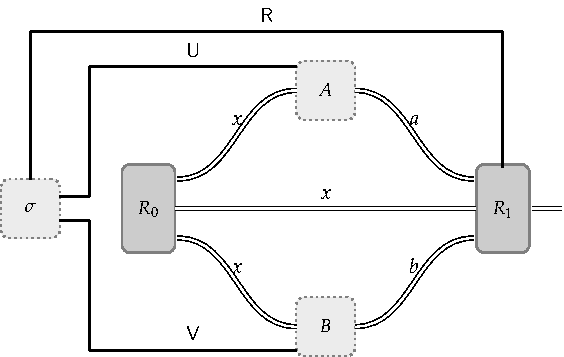
\includegraphics[scale=0.9]{figures/moe_2.pdf}
	\end{center}
		\caption[A monogamy-of-entanglement game.]{A monogamy-of-entanglement game. The state $\sigma \in \Density(\U \otimes \R \otimes \V)$ contained in registers $(\reg{U},\reg{R},\reg{V})$ is prepared by Alice and Bob, where $\reg{R}$ is sent to the referee and $\reg{U}$ belongs to Alice and $\reg{V}$ belongs to Bob. The referee selects question $x$ according to the $\pi$ distribution, and sends $x$ to both Alice and Bob. Alice and Bob then generate and send answers $a$ and $b$ to the referee. Alice and Bob win if and only if all measurement outcomes agree. }
		\label{fig:monogamy-game}
\end{figure}

%-------------------------------------------------------------------------------
\subsection{Strategies and values of monogamy-of-entanglement games}
%-------------------------------------------------------------------------------
Since monogamy-of-entanglement games are a type of extended nonlocal game, one may also define unentangled strategies, standard quantum strategies, commuting measurement strategies, and non-signaling strategies as considered in Chapter~\ref{chap:extended_nonlocal_games} in a similar manner. We shall define some of these strategies and their corresponding values for the case of monogamy-of-entanglement games explicitly. 

For instance, a \index{standard quantum strategy (monogamy-of-entanglement game)}{\emph{standard quantum strategy}} for a monogamy-of-entanglement game consists of finite-dimensional complex Euclidean spaces $\U$ for Alice and $\V$ for Bob, a quantum state $\sigma \in \Density(\U \otimes \R \otimes \V)$, and two collections of measurements 
\begin{align}
	\{ A_a^x : a \in \Gamma \} \subset \Pos(\U) \quad \textnormal{and} \quad \{ B_a^x : a \in \Gamma \} \subset \Pos(\V),
\end{align}
for each $x \in \Sigma$. The measurement operators satisfy the constraint that 
\begin{align}
	\sum_{a \in \Gamma} A_a^x = \I_{\U} \quad \textnormal{and} \quad \sum_{a \in \Gamma} B_a^x = \I_{\V},
\end{align}
for each $x \in \Sigma$. 
For a monogamy-of-entanglement game, the winning probability for Alice and Bob when they use a standard quantum strategy is given by 
\begin{align}
	\sum_{x \in \Sigma} \pi(x) \sum_{a \in \Gamma} \biggip{A_a^x \otimes R(a|x) \otimes B_a^x}{\sigma}.
\end{align}
In fact, we may simplify the above expression slightly. Recall from Section~\ref{sec:standard-quantum-strategies-extended-nonlocal-games} that we may assume that $\sigma \in \Density(\U \otimes \R \otimes \V)$ is pure for any extended nonlocal game, and the measurements of the referee are positive semidefinite, it follows by convexity that we may write the winning probability for Alice and Bob when they use a standard quantum strategy as 
\begin{align} \label{eq:monogamy-ent-val}
	\biggnorm{\sum_{x \in \Sigma} \pi(x) \sum_{a \in \Gamma} A_a^x \otimes R(a|x) \otimes B_a^x }.
\end{align}
For a given monogamy-of-entanglement game $G = (\pi,R)$, we write $\omega^*(G)$ to denote the standard quantum value of $G$, which is the supremum winning value of Alice and Bob's winning probability over all standard quantum strategies for $G$. 

An \index{unentangled strategy (monogamy-of-entanglement game)}{\emph{unentangled strategy}} for a monogamy-of-entanglement game is simply a standard quantum strategy for which the state $\sigma \in \Density(\U \otimes \R \otimes \V)$ initially prepared by Alice and Bob is fully separable. The unentangled value of a monogamy-of-entanglement game, $G$, can be directly derived from the unentangled value of an extended nonlocal game from equation~\eqref{eq:enlg-unentangled-value} as 
\begin{align} \label{eq:monogamy-unentangled-value}
	\omega(G) = \max_{f : \Sigma \rightarrow \Gamma} \biggnorm{\sum_{x \in \Sigma} \pi(x) R(f(x)|x) },
\end{align}
noting again that Alice and Bob only win in a monogamy-of-entanglement game when their measurement outcomes agree with the measurement outcome of the referee. 

A \index{non-signaling strategy (monogamy-of-entanglement game)}{\emph{non-signaling strategy}} for a monogamy-of-entanglement game consists of a non-signaling assemblage $K : \Gamma \times \Sigma \rightarrow \Pos(\R)$ such that 
\begin{align}
	\sum_{a \in \Gamma} K(a,b|x,y) = \xi_b^y \quad \textnormal{and} \quad \sum_{b \in \Gamma} K(a,b|x,y) = \rho_a^x,
\end{align}
for all $x \in \Sigma$ and $y \in \Sigma$ where $\{\xi_b^y : y \in \Sigma, \ b \in \Gamma \}$ and $\{ \rho_a^x : x \in \Sigma, \ a \in \Gamma \}$ are collections of operators satisfying 
\begin{align}
	\sum_{a \in \Gamma} \rho_a^x = \tau = \sum_{b \in \Gamma} \xi_b^y,
\end{align}
for all $x \in \Sigma$ and $y \in \Sigma$ and where $\tau \in \Density(\R)$ is a density operator. For any monogamy-of-entanglement game the winning probability when Alice and Bob use a non-signaling strategy is given by 
\begin{align}
	\sum_{x \in \Sigma} \pi(x) \sum_{a \in \Gamma} \biggip{R(a|x)}{K(a,a|x,x)}.
\end{align}
For a monogamy-of-entanglement game, $G$, the non-signaling value, $\omega_{\ns}(G)$ is the supremum value of the winning probability of $G$ taken over all non-signaling strategies for Alice and Bob.



%-------------------------------------------------------------------------------
\subsection{The BB84 monogamy-of-entanglement game} \label{sec:the-bb84-monogamy-of-entanglement-game}
%-------------------------------------------------------------------------------

In the following example, we shall consider one type of monogamy-of-entanglement game referred to as the \index{BB84 monogamy-of-entanglement game}{\emph{BB84 monogamy-of-entanglement game}}, denoted as $G_{\BB84}$ for short. As we shall see, the name of the game comes from the sets of measurements that the referee uses, which are defined from the BB84 measurement operators~\cite{Bennett1984}. This game was initially introduced and studied in~\cite{Tomamichel2013}. Note that we also already previously considered this game in Chapter~\ref{chap:extended_npa_hierarchy} when we looked at the examples found in Sections~\ref{sec:examples-upper-bounds-extended-npa} and~\ref{sec:examples-lower-bounds}.
%% Example: BB84 game
\begin{example}[BB84 monogamy-of-entanglement game~\cite{Tomamichel2013}]\label{ex:bb84-monogamy-game}
	Let $\Sigma = \Gamma = \{0,1\}$, define 
		\begin{equation} \label{eq:bb84-meas-ops}
	\begin{aligned}
		R(0|0) &= E_{0,0} = \begin{pmatrix} 1 & 0 \\ 0 & 0 \end{pmatrix}, \\
		R(1|0) &= E_{1,1} = \begin{pmatrix} 0 & 0 \\ 0 & 1 \end{pmatrix}, \\
		R(0|1) &= \frac{1}{2}\left( E_{0,0} + E_{0,1} + E_{1,0} + E_{1,1} \right) = \begin{pmatrix} \frac{1}{2} & \frac{1}{2} \\ \frac{1}{2} & \frac{1}{2} \end{pmatrix} , \\
		R(1|1) &= \frac{1}{2}\left( E_{0,0} - E_{0,1} - E_{1,0} + E_{1,1} \right) = \begin{pmatrix} \frac{1}{2} & -\frac{1}{2} \\ -\frac{1}{2} & \frac{1}{2} \end{pmatrix},
	\end{aligned}
	\end{equation}
	and define $\pi(0) = \pi(1) = 1/2$. Then the BB84 monogamy-of-entanglement game, denoted as $G_{\BB84}$, is specified by $G_{\BB84} = (\pi,R)$. 
\end{example}
In~\cite{Tomamichel2013}, the authors also showed that even if Alice and Bob adopt a standard quantum strategy for $G_{\BB84}$, they will perform \emph{no better} than had they simply used an unentangled strategy, 
\begin{align}
	\omega(G_{\BB84}) = \omega^*(G_{\BB84}) = \cos^2(\pi/8) \approx 0.8536.
\end{align}  
That is to say, Alice and Bob gain no advantage in sharing entanglement with the referee. Recall that in Sections~\ref{sec:examples-upper-bounds-extended-npa} and~\ref{sec:examples-lower-bounds}, we computed the lower and upper bound on the standard quantum value of $G_{\BB84}$ and found that both values agree and are equal to $\cos^2(\pi/8)$. 

%\comment{TODO}
%To observe $\omega(G_{\BB84}) = \cos^2(\pi/8)$, we can use equation~\eqref{eq:monogamy-unentangled-value} to show
%\begin{equation}
%	\begin{aligned}
%		\omega(G_{\BB84}) &= \max_{f : \Sigma \rightarrow \Gamma} \biggnorm{\frac{1}{2} R(f(x)|0) + \frac{1}{2} R(f(x)|1)} \\
%		&= \frac{1}{2} \biggnorm{R(0|0) + R(0|1)} + \frac{1}{2} \biggnorm{R(1|0) + R(1|1)} \\
%		&= \frac{1}{2} + \frac{1}{2 \sqrt{2}} = \cos^2(\pi/8).
%	\end{aligned}
%\end{equation} 
%
%To show that $\omega^*(G_{\BB84}) = \cos^2(\pi/8)$, we consider the following standard quantum strategy. Alice and Bob prepare the state 
%\begin{align}
%	u = \cos(\pi/8)e_0 + \sin(\pi/8)e_1,
%\end{align}
%and send it to the referee. Alice and Bob then always output $a = 0$, regardless of what the question $x$ sent by the referee is. Define the state 
%\begin{align}
%	v_{\pm} = \cos(\pi/8)e_0 \pm \sin(\pi/8)e_1,
%\end{align}
%and define 
%\begin{align}
%	A_0^0 = v_+ v_+^*, \quad A_0^1 = v_- v_-^*, \quad B_0^0 = B_0^1 = \I_{\B}
%\end{align}
%to be the measurement operators for Alice and Bob. By using equation~\eqref{eq:monogamy-ent-val}, observe that 
%\begin{equation}
%	\begin{aligned}
%		\omega^*(G_{\BB84}) &= \biggnorm{ \frac{1}{2} \left(R(0|0) \otimes A_0^0 \otimes B_0^0 + R(1|0) \otimes A_0^0 \otimes B_0^0\right) \\
%		& \ \ + \frac{1}{2} \left( R(0|1) \otimes A_0^1 \otimes B_0^1 + R(1|1) \otimes A_0^1 \otimes B_0^1 \right) } \\
%		&= \cos^2(\pi/8).
%	\end{aligned}
%\end{equation}
%The optimality of this strategy follows from the result of~\cite{Tomamichel2013}. 
%\comment{END TODO}

%Furthermore, it was also shown in~\cite{Tomamichel2013} that the BB84 game exhibits the property of strong parallel repetition, 
%\begin{align}
%	\omega^*(G_{\BB84}^r) = \omega^*(G_{\BB84})^r = \left( \cos^2(\pi/8) \right)^r,
%\end{align}
%where $r$ is the number of rounds of repetition performed. 

%%We shall defer the proof of this fact until Section~\ref{}, where we prove that 
%
%One may naturally be curious if the properties for $G_{\BB84}$ shown in~\cite{Tomamichel2013} and mentioned above also apply to other classes of monogamy-of-entanglement games. Specifically, 
%
%\begin{question} \label{ques:monog-classical-quantum-vals}
%	For any monogamy-of-entanglement game $G$, is it true that 
%		\begin{align}
%			\omega(G) = \omega^*(G)?
%		\end{align}
%\end{question}
%
%\begin{question} \label{ques:monog-strong-parallel-rep}
%	For any monogamy-of-entanglement game $G$, does strong parallel repetition hold?
%\end{question}
%
%For Question~\ref{ques:monog-classical-quantum-vals}, we show in Section~\ref{sec:monog-classical-quantum} that there does exist a class of monogamy-of-entanglement games where the classical and and quantum values agree for games where $\abs{\Sigma} = 2$ and $\abs{\Gamma} = k$ for any $k \geq 1$. In contrast, we show that there exists a monogamy-of-entanglement game $G$, such that $\omega(G) < \omega^*(G)$ where $\abs{\Sigma} = 4$ and $\abs{\Gamma} = 3$ in Section~\ref{sec:MUB-4-3}.
%
%For Question~\ref{ques:monog-strong-parallel-rep},  

%-------------------------------------------------------------------------------
\subsection{Comparing standard quantum and unentangled strategies for monogamy-of-entanglement games} \label{sec:monog-classical-quantum}
%-------------------------------------------------------------------------------

Recall from Section~\ref{sec:the-bb84-monogamy-of-entanglement-game} that $\omega(G_{\BB84}) = \omega^*(G_{\BB84})$, meaning that it makes no difference whether Alice and Bob adopt a standard quantum or unentangled strategy for $G_{\BB84}$, as they will win with the same probability either way. A natural question then is whether this behavior persists in general for the class of monogamy-of-entanglement games. Specifically, is it the case that for any monogamy-of-entanglement game, $G$, that 
\begin{align}
	\omega(G) = \omega^*(G)?
\end{align}

In this section, we shall show that for any monogamy-of-entanglement game where the size of the question set is two and the size of the answer set is arbitrary, the standard quantum and unentangled values are indeed equal. However, in Section~\ref{sec:MUB-4-3}, we shall show that this behavior is \emph{not true} for the entire class of monogamy-of-entanglement games and present an explicit example of a monogamy-of-entanglement game that yields a strictly higher standard quantum value than unentangled value.  

%% Theorem: Classical / quantum is the same for 2 questions
\begin{theorem}
	Let $G$ be any monogamy-of-entanglement game for which the question set $\Sigma$ satisfies $\abs{\Sigma}=2$. It holds that 
	\begin{align}
		\omega(G) = \omega^*(G).
	\end{align}
\end{theorem}

%% Proof: Classical / quantum is the same for 2 questions
\begin{proof}
	It is evident that $\omega(G) \leq \omega^*(G)$, as this is the case for every extended nonlocal game (and therefore every monogamy-of-entanglement game), so it remains to prove the reverse inequality. 
	Assume without loss of generality that $\Sigma = \{0,1\}$, and that $G = (\pi,R)$ for $\pi(0) = \lambda$ and $\pi(1) = 1 - \lambda$. Consider any choice of projective measurements 
	\begin{align}
		\left \{ A_a^0 : a \in \Gamma \right \} \quad \textnormal{and} \quad \left \{ A_a^1 : a \in \Gamma  \right \}
	\end{align}
on $\U$ for Alice and 
	\begin{align}
		\left \{ B_a^0 : a \in \Gamma \right \} \quad \textnormal{and} \quad \left \{ B_a^1 : a \in \Gamma \right \}
	\end{align}
on $\V$ for Bob. First, note that for an optimal choice of the initial state, we can write the standard quantum value of $G$ in terms of the following equation 
	\begin{align} \label{eq:classical-quantum-monogamy}
		\omega^*(G) = \biggnorm{\lambda \sum_{a \in \Gamma} A_a^0 \otimes R(a|0) \otimes B_a^0 + (1-\lambda) \sum_{b \in \Gamma}  A_b^1 \otimes R(b|1) \otimes B_b^1 }.
	\end{align}
Note that the operator inside the norm of equation~\eqref{eq:classical-quantum-monogamy} is positive semidefinite since all of the measurement operators are also positive semidefinite. 

Recall that for positive semidefinite operators $P \in \Pos(\U)$ and $Q \in \Pos(\V)$ that if $P \leq Q$ then it implies that $\norm{P} \leq \norm{Q}$. To observe this fact, note that for a positive semidefinite operator, $X$, the spectral norm yields the largest eigenvalue of that operator. An equivalent way to state that $X$ is positive semidefinite is to say that $X$ is Hermitian with nonnegative eigenvalues. 

%Due to the monotonicity theorem, all eigenvalues of $X$ increase if a positive semidefinite matrix is added to it. 

We can, therefore, upper bound $\omega^*(G)$ in the following way 
\begin{align} \label{eq:classical-quantum-monogamy-identity}
	\omega^*(G) \leq \biggnorm{\lambda \sum_{a \in \Gamma} A_a^0 \otimes  R(a|0) \otimes \I_{\V} + (1 - \lambda) \sum_{b \in \Gamma} \I_{\U} \otimes R(b|1) \otimes B_b^1}.
\end{align}
Since we enforce that the operators $A_a^x$ and $B_b^y$ are valid measurement operators, it holds that 
\begin{align}
	\sum_{a \in \Gamma} A_a^x = \I_{\U} \quad \textnormal{and} \quad \sum_{b \in \Gamma} B_b^y = \I_{\V}
\end{align}
for all $x \in \Sigma$ and $y \in \Sigma$. Let us now replace the identity operators from equation~\eqref{eq:classical-quantum-monogamy-identity} with these sums to obtain
\begin{align}
	\omega^*(G) \leq \biggnorm{\lambda \sum_{a,b \in \Gamma} A_a^0 \otimes R(a|0) \otimes B_b^1 + (1 - \lambda) \sum_{a,b \in \Gamma} A_a^0 \otimes R(b|1) \otimes B_b^1}.
\end{align}
Since $\{A_a^0 \otimes B_b^1 : a,b \in \Gamma\}$ are pairwise orthogonal projections, i.e. that $\ip{A_a^0 \otimes B_b^1}{A_{a^{\prime}}^0 \otimes B_{b^{\prime}}^1} = 0$ for $a \not= a^{\prime}$ and $b \not= b^{\prime}$ and also that it holds that 
\begin{align}
	\biggnorm{\sum_{k} A_k \otimes \Pi_k} = \max_k \norm{A_k}
\end{align}
for a projective measurement $\{\Pi_k\}$, we have that 
\begin{align}
	\biggnorm{\sum_{(a,b) \in \Gamma} A_a^0 \otimes \left( \lambda R(a|0) + (1-\lambda) R(b|1) \right) \otimes B_b^1 } \leq \max_{a,b \in \Gamma} \biggnorm{ \lambda R(a|0) + (1-\lambda)R(b|1) }.
\end{align}
It follows from equation~\eqref{eq:monogamy-unentangled-value} that 
\begin{align}
	\omega(G) = \max_{a,b \in \Gamma} \biggnorm{ \lambda R(a|0) + (1-\lambda) R(b|1) }.
\end{align}
Therefore $\omega^*(G) \leq \omega(G)$.

\end{proof}

%-------------------------------------------------------------------------------
\section{Parallel repetition of monogamy-of-entanglement games} \label{sec:parallel-rep-moe-games}
%-------------------------------------------------------------------------------

For an integer $r \geq 1$ and some monogamy-of-entanglement game, $G$, the \index{parallel repetition}{\emph{$r$-fold parallel repetition}} of a monogamy-of-entanglement game is when Alice and Bob play $r$ copies of $G$, denoted as $G^r$, wherein the referee gives the players $r$ independent and identically distributed pairs of questions simultaneously and expects a response from Alice and Bob for each instance. The referee accepts if and only if all of the $r$ responses satisfy the criteria for the initial game, and rejects otherwise. The parallel repetition of a monogamy-of-entanglement game is depicted in Figure~\ref{fig:parallel-rep-monogamy-game}. 

Define the complex Euclidean spaces $\R_1, \ldots, \R_r$ and define alphabets 
\begin{align}
	\Sigma = \Sigma_1 \times \cdots \times \Sigma_r \quad \textnormal{and} \quad \Gamma = \Gamma_1 \times \cdots \times \Gamma_r
\end{align}
such that $x_1 \in \Sigma_1, \ldots, x_r \in \Sigma_r$ are selected from $\Sigma$ according to 
\begin{align}
	\pi^k : \Sigma_1 \times \cdots \times \Sigma_k \rightarrow [0,1]
\end{align}
where $\pi^k(x_1, \ldots, x_r) = \pi(x_1) \cdots \pi(x_r)$. Then the $r$-fold parallel repetition of $G$ starts off with the referee accepting $r$ registers $\reg{R}_1, \ldots, \reg{R}_r$ from Alice and Bob where the contents of the registers correspond to the state 
\begin{align}
	\sigma \in \Density(\U \otimes \R_1 \otimes \cdots \otimes \R_r \otimes \V),
\end{align}
and selecting $r$ questions $x_1 \in \Sigma, \ldots, x_r \in \Sigma$ according to $\pi$. The referee then sends $x_1, \ldots, x_r$ to Alice and Bob. The players return $r$ answers $a_1 \in \Gamma_1, \ldots, a_r \in \Gamma_r$ for each question. The referee then performs a measurement from the set 
\begin{align} \label{eq:monog-parallel-rep-ref-ops}
	\left \{ R(a_1, \ldots, a_r|x_1, \ldots, x_r) = R(a_1|x_1) \otimes \cdots \otimes R(a_r|x_r) : a_i \in \Gamma, \ x_i \in \Sigma \right \}.
\end{align}
Alice and Bob win the parallel repetition of $G$ if and only if their answers win each of the $r$ instances of $G^r$. That is, for a monogamy-of-entanglement game, Alice and Bob win if and only if the outcomes of their measurements in every $r$ instance of the game matches with the referee's measurement outcome for every $r$ games. 

\begin{figure}[!htpb] 
	\begin{center}
		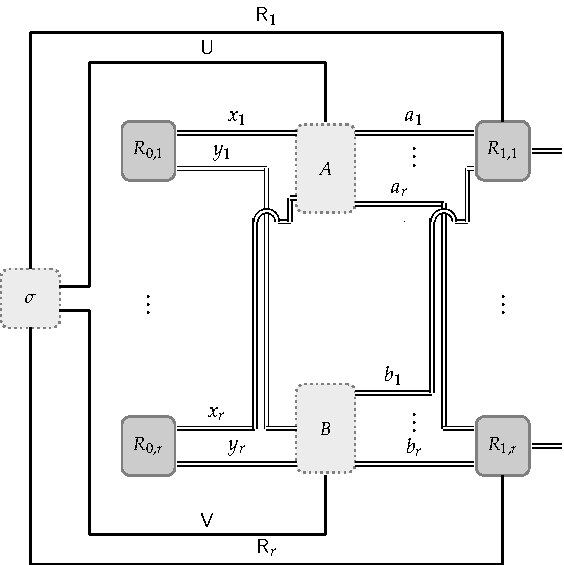
\includegraphics[scale=0.9]{figures/extended_nonlocal_game_parallel_repetition_2.pdf}
	\end{center}
		\caption[Parallel repetition of a monogamy-of-entanglement game.]{Parallel repetition of a monogamy-of-entanglement game. Alice and Bob prepare registers $(\reg{R}_1, \ldots, \reg{R}_r)$ and send to the referee. The referee then asks questions $x_1, \ldots, x_r$ to Alice and $y_1, \ldots, y_r$ to Bob. Alice and Bob respond to each question with answers $a_1, \ldots, a_r$ and $b_1, \ldots, b_r$. Once the referee receives all the answers, it performs a measurement. Alice and Bob win the parallel repetition of the monogamy-of-entanglement game if and only if all their answers match the referee's measurement outcome for every $r$ instance.}
		\label{fig:parallel-rep-monogamy-game}
\end{figure}

One may ask how $\omega(G^r)$ depends on $\omega(G)$ and $r$. It is evident that $\omega(G^r) \geq \omega(G)^r$ since Alice and Bob can simply perform the same strategy in each instance. For any game that has the property $\omega(G) = 1$, it holds that $\omega(G^r) = 1$ for any $r$. One may also wish to ask the question of how $\omega(G^r)$ scales in the event that $\omega(G) < 1$. First note that $\omega(G^r) \leq \omega(G)$. This can be seen since, in order for the players to win all instances of the game, they must win the original game, $G$. Note also that $\omega(G)^r \leq \omega(G^r)$ and $\omega(G)^r \leq \omega(G)$. This holds since the players can simply play each game independently with the optimal strategy for the original game. We, therefore, have the following inequality relationship for the parallel repetition of $G$\
\begin{align}
	\omega(G)^r \leq \omega(G^r) \leq \omega(G). 
\end{align} 
It may be tempting to conclude that $\omega(G^r) = \omega(G)^r$ for all games, however this was surprisingly disproven~\cite{Fortnow1990, Feige1991, Verbitsky1996, Feige2002}. Specifically in~\cite{Fortnow1990}, Fortnow introduced a game $G$ for which $\omega(G^2) > \omega(G)^2$. This result was later improved by Feige~\cite{Feige1991}, by exhibiting an example of a game where $\omega(G^2) = \omega(G)$ with $\omega(G) < 1$.  

We say that a game $G$ exhibits the property of \index{strong parallel repetition}{\emph{strong parallel repetition}} if the value of the game raised to the $r$ power is equal to the value of running the game $r$ times. For instance, a monogamy-of-entanglement game, $G$, where the players use a standard quantum strategy satisfies strong parallel repetition if and only if
\begin{align}
	\omega^*(G^r) = \omega^*(G)^r. 
\end{align}
Strong parallel repetition has been also referred to as perfect parallel repetition elsewhere in the literature as in~\cite{Cleve2008}. 

It is a fact proved in~\cite{Tomamichel2013} that the BB84 game, $G_{\BB84}$, exhibits the property of strong parallel repetition,
\begin{align}
	\omega^*(G_{\BB84}^r) = \omega^*(G_{\BB84})^r = \left( \cos^2(\pi/8) \right)^r,
\end{align}
where $r$ is the number of rounds of repetition performed. A natural question for the general class of monogamy-of-entanglement games might be whether this behavior holds for any monogamy-of-entanglement game. In Section~\ref{sec:monog-strong-parallel-rep}, we prove that for any monogamy-of-entanglement game $G = (\pi,R)$ where the set of measurements belonging to the referee, $R$, are projective, the distribution $\pi$ is uniform, the size of the question set is $\abs{\Sigma} = 2$, and the size of the answer set is $\abs{\Gamma} = k$ for some integer $k \geq 1$, then strong parallel repetition holds. 

This result of strong parallel repetition holds for the case when Alice and Bob use either an unentangled or a standard quantum strategy since we know from Section~\ref{sec:monog-classical-quantum} that 
\begin{align}
	\omega(G) = \omega^*(G)
\end{align}
for any monogamy-of-entanglement game $G$, with $\abs{\Sigma} = 2$ and $\abs{\Gamma} = k$ for some integer $k \geq 1$. Specifically, the result that is shown in Section~\ref{sec:monog-strong-parallel-rep} is that 
\begin{align}
	\omega(G^r) = \omega(G)^r \quad \textnormal{and} \quad \omega^*(G^r) = \omega^*(G)^r,
\end{align}
where $r$ is the number of repetitions and $G = (\pi,R)$ is a monogamy-of-entanglement where $\abs{\Sigma} = 2$, $\abs{\Gamma} = k$, $\pi$ is uniform, and $R$ is a collection of projective measurement operators. 

While strong parallel repetition holds for a specific class of monogamy-of-entanglement games when Alice and Bob use either an unentangled or standard quantum strategy, we can ask a similar question when Alice and Bob use a non-signaling strategy instead. As we shall see in Section~\ref{sec:monog-non-signaling}, it turns out that strong parallel repetition does \emph{not} hold in the non-signaling scenario. We shall illustrate this by showing a counter-example to strong parallel repetition by using a non-signaling version of the BB84 monogamy-of-entanglement game and showing that
\begin{align}
	\omega_{\ns}(G_{\BB84}^r) \not= \omega_{\ns}(G_{\BB84})^r.
\end{align}
for $r = 2$. 

%-------------------------------------------------------------------------------
\subsection{Strong parallel repetition for certain monogamy-of-entanglement games with two questions} \label{sec:monog-strong-parallel-rep}
%-------------------------------------------------------------------------------

We begin this section by recalling a theorem from~\cite{Tomamichel2013}.

\begin{theorem}[Tomamichel, Fehr, Kaniewski, and Wehner (Theorem 4 of~\cite{Tomamichel2013})] \label{thm:parallel-rep-monogamy-bound}
	Let $G = (\pi,R)$ be a monogamy-of-entanglement game for which $\pi$ is uniform over $\Sigma$, define 
	\begin{align} \label{eq:monog-c-g}
		c(G) = \max_{\substack{x,y \in \Sigma \\ x \not= y}} \max_{a,b \in \Gamma} \biggnorm{\sqrt{R(a|x)} \sqrt{R(b|y)}}^2, 
	\end{align}
	and let $G^r$ denote the game played $r$ times in parallel. It holds that 
	\begin{align} \label{eq:monog-tfkw-bound}
		\omega^*(G^r) \leq \left( \frac{1}{\abs{\Sigma}} + \frac{\abs{\Sigma} - 1}{\abs{\Sigma}} \sqrt{c(G)} \right)^r.
	\end{align}
\end{theorem}

Equation~\eqref{eq:monog-c-g} may be referred to as the maximal overlap of the referee's measurements. As was observed in~\cite{Tomamichel2013}, this quantity satisfies
\begin{align}
	\frac{1}{\abs{\Gamma}} \leq c(G) \leq 1 \quad \textnormal{and} \quad c(G^r) = c(G)^r. 
\end{align}
For any monogamy-of-entanglement game, $G$, Theorem~\ref{thm:parallel-rep-monogamy-bound} provides an upper bound on the standard quantum value achieved when running $G$ for $r$ times in parallel as given by equation~\eqref{eq:monog-tfkw-bound}. In this section, we shall show that for $\abs{\Sigma} = 2$ that the bound from equation~\eqref{eq:monog-tfkw-bound} is indeed tight. 

\begin{theorem} \label{thm:monog-parallel-rep-2}
	Let $G = (\pi,R)$ be a monogamy-of-entanglement game for which $\pi$ is uniform over $\Sigma$ with $\abs{\Sigma} = 2$. It holds that 
	\begin{align}
	\omega^*(G^r) = \left(\frac{1}{2} + \frac{1}{2} \sqrt{c(G)} \right)^r.
\end{align}
\end{theorem}

In order to prove theorem~\ref{thm:monog-parallel-rep-2}, we first require the following proposition. 
\begin{prop} \label{prop:monogamy-unentangled}
	Let $G = (\pi,R)$ be a monogamy-of-entanglement game for which $\Sigma = \{0,1\}$, $\pi$ is uniform over $\Sigma$, and $R(a|x)$ is a projection operator for each $x \in \Sigma$ and $a \in \Gamma$. It holds that 
	\begin{align}
		\omega(G) = \frac{1}{2} + \frac{1}{2} \max_{a,b \in \Gamma} \biggnorm{R(a|0)R(b|1)}.
	\end{align}
\end{prop}
Proving this proposition requires the use of the following lemma.
\begin{lemma} \label{lem:monogamy-projections}
	Let $\Pi_0$ and $\Pi_1$ be nonzero projection operators on $\complex^r$. It holds that 
	\begin{align}
		\bignorm{\Pi_0 + \Pi_1} = 1 + \bignorm{\Pi_0 \Pi_1}.
	\end{align}
\end{lemma}

\begin{proof}
	For every choice of unit vectors $u_0, u_1 \in \complex^r$, one has the formula
	\begin{align}
		\bignorm{ u_0 u_0^* + u_1 u_1^* } = 1 + \abs{\ip{u_0}{u_1}},
	\end{align}
	which follows from the observation that the Hermitian operator $u_0 u_0^* + u_1 u_1^*$ has (at most) two nonzero eigenvalues $1 \pm \abs{\ip{u_0}{u_1}}$. Letting $\S$, $\S_0$, and $\S_1$ denote the unit spheres in the spaces $\complex^r$, $\im(\Pi_0)$, and $\im(\Pi_1)$, respectively, one has 
	\begin{equation}
		\begin{aligned}
			\bignorm{\Pi_0 + \Pi_1} &= \max \left \{ v^* \left( \Pi_0 + \Pi_1 \right) v : v \in \S \right \} \\
			&= \max \left \{ \bignorm{\Pi_0 v}^2 + \bignorm{\Pi_1 v}^2 : v \in \S \right \} \\
			&= \max \left \{ \abs{\ip{u_0}{v}}^2 + \abs{\ip{u_1}{v}}^2 : v \in \S, \ u_0 \in \S_0, \ u_1 \in \S_1 \right \} \\
			&= \max \left \{ v^* \left( u_0 u_0^* + u_1 u_1^* \right)v : v \in \S, \ u_0 \in \S_0, \ u_1 \in \S_1 \right \} \\
			&= \max \left \{ \bignorm{u_0 u_0^* + u_1 u_1^*} : u_0 \in \S_0, \ u_1 \in \S_1 \right \} \\
			&= \max \left \{ 1 + \abs{\ip{u_0}{u_1}} : u_0 \in \S_0, \ u_1 \in \S_1 \right \} \\
			&= 1 + \bignorm{\Pi_0 \Pi_1},
		\end{aligned}
	\end{equation}
which proves the lemma. 
\end{proof}

%% OLD PROOF OF LEMMA
%% Refer to page 431 of Matrix Analysis and Application in Linear Algebra. 
%\begin{proof}
%	For every choice of unit vectors $u_0, u_1 \in \complex^r$, one has the formula
%	\begin{align}
%		\norm{u_0 u_0^* + u_1 u_1^*} = 1 + \abs{\ip{u_0}{u_1}},
%	\end{align}
%	which follows from the observation that the Hermitian operator $u_0 u_0^* + u_1 u_1^*$ has at most two nonzero eigenvalues $1 \pm \abs{\ip{u_0}{u_1}}$. Letting $\S,\S_0$ and $\S_1$ denote the unit spheres in the spaces $\complex^r$, $\im(\Pi_0)$, and $\im(\Pi_1)$, respectively, it holds that
%	\begin{align} \label{eq:monog-proj-norm-rep}
%		\norm{\Pi_0 + \Pi_1} = \max \Bigl\{ v^*(\Pi_0 + \Pi_1)v : v \in \S \Bigr\}.
%	\end{align}
%Observe that 
%\begin{align}
%	v^*(\Pi_0 + \Pi_1)v = v^* \Pi_0 v	+ v^* \Pi_1 v = \norm{\Pi_0 v}^2 + \norm{\Pi_1 v}^2.
%\end{align}	
%We may therefore write equation~\eqref{eq:monog-proj-norm-rep} as 
%\begin{align}
%	\max \Bigl \{ \norm{\Pi_0 v}^2 + \norm{\Pi_1 v}^2 : v \in \S \Bigr \}.
%\end{align}
%Note that we can write 
%\begin{align}
%	\norm{\Pi_0 v}^2 = \max \{ \abs{u^* \Pi_0 v}^2 : u \in \S \}
%\end{align}
%and similarly for $\norm{\Pi_1 v}^2$. It holds that 
%\begin{align}
%	\norm{\Pi_0 v} = \max_{u \in \S} \abs{\ip{u}{\Pi_0 v}}.
%\end{align}
%It follows from Cauchy-Schwartz that 
%\begin{align}
%	\abs{\ip{u}{\Pi_0 v}} \leq \norm{u} \norm{\Pi_0 v} = \norm{\Pi_0 v}.
%\end{align}
%Furthermore, equality in the above expression is achieved when 
%\begin{align}
%	u = \frac{\Pi_0 v}{\norm{\Pi_0 v}},
%\end{align}
%as can be seen by 
%\begin{align}
%	\frac{\abs{\ip{\Pi_0 v}{\Pi_0 v}}}{\norm{\Pi_0 v}} = \frac{\norm{\Pi_0 v}^2}{\norm{\Pi_0 v}} = \norm{\Pi_0 v}.
%\end{align}
%Taking the set 
%\begin{align}
%	\{ \Pi_0 u : u \in \S \} = \{ z \in \im(\Pi_0) : \norm{z} \leq 1 \},
%\end{align}
%we may write 
%\begin{align}
%	u = u_0 + u_1,
%\end{align}
%where $u_0 \in \im(\Pi_0)$ and $u_1 \in \im(\Pi_1)$. This allows us to write equation~\eqref{eq:monog-proj-norm-rep} as 
%\begin{align}
%	\max \Bigl\{ \abs{ \ip{u_0}{v} }^2 + \abs{ \ip{u_1}{v} }^2 : v \in \S, u_0 \in \S_0, u_1 \in \S_1 \Bigr\},
%\end{align}
%where again $\S_0$ denotes the unit sphere in the space of $\im(\Pi_0)$ and $\S_1$ denotes the unit sphere in the space of $\im(\Pi_1)$.
%%XXX
%%\comment{TODO: Still need to check this part (Start)}
%%By using the Cauchy-Schwarz inequality, we have that 
%%\begin{align}
%%	\abs{\ip{u_0}{v}} \leq \norm{u_0} \norm{v} \quad \textnormal{and} \quad \abs{\ip{u_1}{v}} \leq \norm{u_1} \norm{v},
%%\end{align}
%%where equality is achieved since $u_0$ and $v$ are linearly dependent, and so are $u_1$ and $v$. Since $v$ is a unit eigenvector of the operator $u_0 u_0^* + u_1 u_1^*$ that corresponds to the largest eigenvalue, which gives us 
%%\begin{align}
%%	v^*(u_0 u_0^* + u_1 u_1^*)v = \norm{u_0 u_0^* + u_1 u_1^*}. 
%%\end{align}
%%We may then write equation~\eqref{eq:monog-proj-norm-rep} as 
%It is evident that 
%\begin{align}
%	\abs{\ip{u_0}{v}}^2 = v^* u_0 u_0^* v
%\end{align}
%for all $u_0$ and for all $v$. We may then write equation~\eqref{eq:monog-proj-norm-rep} as 
%\begin{align}
%	\max \Bigl \{ v^*(u_0 u_0^* + u_1 u_1^*)v : v \in \S, u_0 \in \S_0, u_1 \in \S_1 \Bigr \}.
%\end{align}
%%XXX
%%\comment{TODO: Still need to check this part (End)}
%This allows us to write equation~\eqref{eq:monog-proj-norm-rep} as 
%\begin{align}
%	\max \Bigl \{ \norm{u_0 u_0^* + u_1 u_1^*} : u_0 \in \S_0, u_1 \in \S_1 \Bigr \}.
%\end{align}
%Note that for every choice of unit vectors $u_0, u_1 \in \complex^r$, one has that 
%\begin{align}
%	\norm{u_0 u_0^* + u_1 u_1^*} = 1 + \abs{\ip{u_0}{u_1}},
%\end{align}
%%which follows from the observation that the Hermitian operator $u_0 u_0^* + u_1 u_1^*$ has at most two nonzero eigenvalues $1 \pm \abs{\ip{u_0}{u_1}}$.
%We may therefore write equation~\eqref{eq:monog-proj-norm-rep} as 
%\begin{align}
%	\max \Bigl \{ 1 + \abs{\ip{u_0}{u_1}} : u_0 \in \S_0, u_1 \in \S_1 \Bigr \}.
%\end{align}
%%Finally, since for every operator $A \in \Lin(\X,\Y)$ it holds from the duality of the the Schatten $p$-norm and $p^*$-norm that
%%\begin{align}
%%	\norm{A}_p = \max \Bigr \{ \abs{\ip{B}{A}} : B \in \Lin(\X,\Y), \norm{B}_{p^*} \leq 1  \Bigl \}. 
%%\end{align}
%We may therefore write equation~\eqref{eq:monog-proj-norm-rep} as 
%\begin{align}
%	1 + \norm{\Pi_0 \Pi_1},
%\end{align}
%which proves the lemma. 
%
%\end{proof}

\begin{proof}[Proof of Proposition~\ref{prop:monogamy-unentangled}]
	From equation~\eqref{eq:enlg-unentangled-value}, we have that the unentangled value of the game $G$ is given by 
	\begin{align} \label{eq:monog-parallel-rep-proj}
		\omega(G) = \max_{a,b \in \Gamma} \biggnorm{\frac{1}{2} R(a|0) + \frac{1}{2} R(b|1) } = \frac{1}{2} \max_{a,b \in \Gamma} \biggnorm{R(a|0) + R(b|1)}.
	\end{align}
	It follows from Lemma~\ref{lem:monogamy-projections} that $\norm{R(a|0) + R(b|1)} = 1 + \norm{R(a|0) R(b|1)}$ which allows us to write equation~\eqref{eq:monog-parallel-rep-proj} as 
	\begin{align}
		\omega(G) = \frac{1}{2} + \frac{1}{2} \max_{a,b \in \Gamma} \biggnorm{R(a|0)R(b|1)},
	\end{align}
	proving the proposition. 
\end{proof}

%% 
\begin{proof}[Proof of Theorem~\ref{thm:monog-parallel-rep-2}]
	The upper bound
		\begin{align}
			\omega^*(G^r) \leq \left(\frac{1}{2} + \frac{1}{2} \sqrt{c(G)} \right)^r,
	\end{align}
	follows from Theorem~\ref{thm:parallel-rep-monogamy-bound}, initially shown in~\cite{Tomamichel2013}. 
	Showing the other direction
		\begin{align}
	\omega^*(G^r) \geq \left(\frac{1}{2} + \frac{1}{2} \sqrt{c(G)} \right)^r,
\end{align}
 follows from Proposition~\ref{prop:monogamy-unentangled} and Lemma~\ref{lem:monogamy-projections}. The reason that this direction holds for any number of repetitions $r$ is that Alice and Bob can simply play an optimal strategy for each $r$ games, $r$ times in parallel. This implies that 
 \begin{align}
 	\omega^*(G^r) \geq \omega(G^r) \geq \left( \frac{1}{2} + \frac{1}{2} \max_{a,b \in \Gamma} \biggnorm{R(a|0)R(b|1)} \right)^r = \left( \frac{1}{2} + \frac{1}{2} \sqrt{c(G)} \right)^r,
 \end{align}
 which matches the upper bound from Theorem~\ref{thm:parallel-rep-monogamy-bound}.
\end{proof}


%-------------------------------------------------------------------------------
\subsection{No strong parallel repetition for monogamy-of-entanglement games with non-signaling provers} \label{sec:monog-non-signaling}
%-------------------------------------------------------------------------------

%% Theorem: No strong parallel repetition for non-signaling
\begin{claim}[No strong parallel repetition for non-signaling provers] \label{thm:no-spr-non-signaling}
	There exists a monogamy-of-entanglement game, $G$, such that
	\begin{align} \label{eq:no-spr-non-signaling}
		\omega_{\ns}(G^2) \not= \omega_{\ns}(G)^2.
	\end{align}		
\end{claim}

\begin{proof}[Proof of Claim~\ref{thm:no-spr-non-signaling}]
	We shall verify equation~\eqref{eq:no-spr-non-signaling} numerically using the convex optimization software CVX~\cite{Grant2008a} in addition to the software listing~\ref{code:ns-counter-example-monogamy-game} in Appendix~\ref{chap:AppendixA}. The explicit monogamy-of-entanglement game that we shall use to verify this claim is $G_{\BB84}$, the BB84 game as mentioned in Section~\ref{sec:the-bb84-monogamy-of-entanglement-game}. It may be checked by running the software listing~\ref{code:ns-counter-example-monogamy-game} that 
	\begin{align}
		\omega_{\ns}(G_{\BB84}^2) \approx 0.73826. 
	\end{align}
However, we may also verify that a single repetition of $G_{\BB84}$ is $\cos^2(\pi/8)$, that is
	\begin{align}
		\omega_{\ns}(G_{\BB84}) = \cos^2(\pi/8).
	\end{align}
From this, it is clear that 
\begin{align}
	\omega_{\ns}(G_{\BB84}^2) \not= \omega_{\ns}(G_{\BB84})^2 = \cos^4(\pi/8),
\end{align}
which concludes the proof. 
\end{proof}

%Prior to proving Theorem~\ref{thm:no-spr-non-signaling}, it will be convenient to consider the following semidefinite programming formulation. Let $\Sigma$ and $\Gamma$ be alphabets such that $n = \abs{\Sigma}$ and $m = \abs{\Gamma}$, let $\X_1, \ldots, \X_n$ and $\Y_1, \ldots, \Y_m$ be complex Euclidean spaces, let $1 \leq k \leq m$ be a positive integer, let $\Phi_k \in \Trans(\X_1 \oplus \ldots \oplus \X_n, \Y_1 \oplus \ldots \oplus \Y_m)$ be a Hermiticity preserving map, and let $A_k \in \Herm(\X_1 \oplus \ldots \oplus \X_n)$ and $B_k \in \Herm(\Y_1 \oplus \ldots \oplus \Y_m)$ be Hermitian operators. Then this form of semidefinite program will be specified by the tuple $(\Phi_k, A_k, B_k)$, and has the following primal problem associated with it
%\begin{center}
%	\centerline{\underline{Primal problem}}\vspace{-7mm}
%		\begin{equation} \label{sdp:ns-sdp-general-primal}
%  		\begin{split}
%      \text{maximize:}\quad & \sum_{k=1}^{n} \ip{A_k}{X_k}\\
%      \text{subject to:}\quad & \Phi_1\left(X_1, \ldots, X_n\right) = B_1,\\
%      & \vdots \\ 
%      & \Phi_m \left(X_1, \ldots, X_n \right) = B_m, \\
%      & X_1 \in \Pos(\X_1), \ldots, X_n \in \Pos(\X_n).
%  		\end{split}
%		\end{equation}
%\end{center}
%We now construct the dual. First, we calculate the dual objective function as
%\begin{align}\label{eq:ns-sdp-general-obj-fun}
%\ip{B_1}{Y_1} + \ldots + \ip{B_m}{Y_m} = \sum_{k=1}^m \ip{B_k}{Y_k}.
%\end{align}
%To calculate the adjoint mapping, $\Phi^*_k$, note that for every $\Phi_k \in \Trans(\X_1 \oplus \ldots \oplus \X_n, \Y_1 \oplus \ldots \Y_m)$, the mapping $\Phi_k^* \in \Trans(\Y_1 \oplus \ldots \oplus \Y_m, \X_1 \oplus \ldots \X_n)$ is the unique mapping for which
%\begin{align}\label{eq:ns-sdp-general-adjoint-formula}
%	\Bigip{\Phi_k^*(Y_1, \ldots, Y_m)}{(X_1, \ldots, X_n)} = \Bigip{(Y_1, \ldots, Y_m)}{\Phi_k(X_1, \ldots, X_n)}
%\end{align}
%for all $(X_1, \ldots, X_n) \in \Lin(\X_1 \oplus \ldots \oplus \X_n)$ and $(Y_1, \ldots, Y_m) \in \Lin(\Y_1 \oplus \ldots \oplus \Y_m)$. For convenience, we denote 
%\begin{align}
%	\Phi \begin{pmatrix}
%					X_1 & \\
%				  & \ddots \\
%				  & & X_n	
%			 \end{pmatrix} \triangleq
%			 \begin{pmatrix}
%			 		\Phi_1(X_1, \ldots, X_n) & \\
%			 		& \ddots \\ 
%			 		& & \Phi_m(X_1, \ldots, X_n) 
%			 \end{pmatrix}.
%\end{align}
%We now use equation~\eqref{eq:ns-sdp-general-adjoint-formula} to calculate the adjoint mapping:
%\begin{equation} \label{eq:ns-sdp-general-adjoint-mapping}
%	\begin{aligned}
%		\left \langle \Phi^* \begin{pmatrix} Y_1 & \\ & \ddots \\ & & Y_m \end{pmatrix}, \begin{pmatrix} X_1 & \\ & \ddots \\ & & X_n \end{pmatrix} \right \rangle &= \left \langle \begin{pmatrix} Y_1 & \\ & \ddots \\ & & Y_m \end{pmatrix}, \Phi \begin{pmatrix} X_1 & \\ & \ddots \\ & & X_n \end{pmatrix} \right \rangle \\
%		&= \sum_{k=1}^m \left \langle Y_k, \Phi_k \begin{pmatrix} X_1 & \\ & \ddots \\ & & X_n \end{pmatrix} \right \rangle \\
%		&= \left \langle \sum_{k=1}^m \Phi^*_k(Y_k), \begin{pmatrix} X_1 & \\ & \ddots \\ & & X_n \end{pmatrix} \right \rangle.
%	\end{aligned}
%\end{equation}
%Using equations~\eqref{eq:ns-sdp-general-obj-fun} and~\eqref{eq:ns-sdp-general-adjoint-formula}, we obtain the corresponding dual problem for the primal problem~\eqref{sdp:ns-sdp-general-primal} as 
%\begin{center}
%	\centerline{\underline{Dual problem}}\vspace{-7mm}
%		\begin{equation} \label{sdp:ns-sdp-general-dual}
%  		\begin{split}
%      \text{minimize:}\quad & \sum_{k=1}^m \ip{B_k}{Y_k} \\
%      \text{subject to:}\quad & \sum_{k=1}^m \Phi_k^*(Y_k) \geq \left(A_1, \ldots, A_n \right), \\
%      & Y_1 \in \Herm(\Y_1), \ldots, Y_m \in \Herm(\Y_m).
%  		\end{split}
%		\end{equation}
%\end{center}
%
%For an arbitrary monogamy-of-entanglement game, $G$, we can calculate $\omega_{\ns}(G)$ by a semidefinite program. By slightly adapting the payoff equation from Section~\ref{sec:non-signaling-strategies-extended-nonlocal-games} for a monogamy-of-entanglement game, we aim to maximize the following quantity
%\begin{align}
%	\sum_{x \in \Sigma} \pi(x) \sum_{(a,b) \in \Gamma} \biggip{R(a|x)}{K(a,a|x,x)},
%\end{align}
%where $\{ R(a|x) : a \in \Gamma \} \subset \Pos(\R)$ are the measurement operators of the referee and the function $K : \Gamma \times \Sigma \rightarrow \Pos(\R)$ is the non-signaling assemblage that satisfies certain constraints which may be written in the following semidefinite program
%\begin{center}
%	\centerline{\underline{Primal problem}}\vspace{-7mm}
%		\begin{equation} \label{sdp:ns-monogamy-game-primal}
%  		\begin{split}
%  			\text{maximize:} \quad & \sum_{x \in \Sigma} \pi(x) \sum_{a \in \Gamma} \bigip{R(a|x)}{K(a,a|x,x)} \\
%    		\text{subject to:} \quad & \sum_{b \in \GammaB} K(a,b|x,y) = \sigma_a^x, \quad \forall a \in \GammaA, \ \forall x,y \in \Sigma,  \\
%    			& \sum_{a \in \GammaA} K(a,b|x,y) = \xi^y_b, \quad \ \forall b \in \GammaB, \ \forall x,y \in \Sigma, \\
%    			& \sum_{a \in \GammaA} \sigma_a^x = \sum_{b \in \GammaB} \xi_b^y = \tau \in \Density(\R).
%  		\end{split}
%		\end{equation}
%\end{center}
%We now construct the dual problem. Using the dual form of equation~\ref{sdp:ns-sdp-general-dual}, we obtain the dual objective function 
%
%\begin{align}
%	\sum_{k=1}^m \ip{B_k}{Y_k} &= \ip{0}{Y_1} + \ip{0}{Y_2} + \ldots + \ip{\tr(\tau)}{Y_m} = \ip{1}{Y_m} = \lambda.
%\end{align}
%We proceed to obtain the dual constraints. Let $X \in \Pos(\R \otimes \A \otimes \B)$ be an operator, and let 
%\begin{align}
%	\left[ X_{\Gamma^*}^{\Sigma^*} \right]_{\Gamma^*}^{\Sigma^*} 	
%\end{align}
%denote the block-matrix whose diagonal consists of sub-block matrices $X^{\Sigma^*}_{\Gamma^*}$ over the sets $\Sigma^*$ and $\Gamma^*$. For some map $\Xi \in \Trans(\X_1 \oplus \ldots \oplus \X_n, \Y_1 \oplus \ldots \oplus \Y_m)$ we have that
%
%\begin{align}
%	\Xi \begin{pmatrix}
%				\left[ \rho_{a,b}^{x,y} \right]_{a,b}^{x,y} & \\
%				& \left[ \sigma_a^x \right]_a^{x,y} \\
%				& & \left[ \xi_b^y \right]_b^{x,y} \\
%				& & & \tau 
%			\end{pmatrix} \triangleq
%			\begin{pmatrix}
%				\left[ S_a^{x,y} \right]_a^{x,y} & \\
%				& \left[ T_b^{x,y} \right]_b^{x,y} \\
%				& & \left[ W^x \right]^{x} \\
%				& & & \left[ Z^y \right]^{y}  \\
%		    & & & & \lambda	
%			\end{pmatrix}
%\end{align}
%
%\noindent where 
%
%\begin{equation}
%	\begin{aligned}
%		S_a^{x,y} = \sum_{b \in \GammaB} K(a,b|x,y) - \sigma_a^x, &\quad W^x = \sum_{a \in \GammaA} \sigma_a^x - \tau, \\ 
%		T_b^{x,y} = \sum_{a \in \GammaA} K(a,b|x,y) - \xi_b^y, &\quad Z^y = \sum_{b \in \GammaB} \xi_b^y - \tau, \quad \lambda = \tr(\tau) \I_{\R}.
%	\end{aligned}
%\end{equation}
%
%\noindent We now construct the adjoint mapping, $\Xi^* \in \Trans(\Y_1 \oplus \ldots \oplus \Y_m, \X_1 \oplus \ldots \oplus \X_n)$, as 
%
%\begin{align}
%	\begin{pmatrix}
%			\left[ S_a^{x,y} + T_b^{x,y} \right]_{a,b}^{x,y} & \\
%			& \left[ -\sum_y S_a^{x,y} + W^x \right]_a^x  \\
%			& & \left[ -\sum_x T_b^{x,y} + Z^y \right]_b^y \\
%			& & & \left[ -W^x - Z^y \right] \\
%			& & & & \lambda
%	\end{pmatrix}.
%\end{align}
%From this, we may write the dual problem as 
%
%%% NOTE:
%% It may either be \lambda/(2*abs(Sigma)) OR \lambda/(\abs(Sigma)\abs(Sigma)). need to check dual for n = 2 to be sure... 
%\begin{center}
%	\centerline{\underline{Dual problem}}\vspace{-7mm}
%		\begin{equation} \label{sdp:ns-monogamy-game-dual}
%  		\begin{split}
%  			\text{minimize:} \quad & \lambda \\
%    		\text{subject to:} \quad & S_a^{x,y} + T_b^{x,y} \geq e_x(y) e_a(b) \pi(x) R(a|x), \quad \forall x,y \in \Sigma, \ \forall a,b \in \Gamma,  \\ 
%    		& W^x \geq \sum_{y \in \SigmaB} S_a^{x,y},  \ \ \ \qquad \quad \qquad \qquad \qquad \forall x \in \SigmaA, \ \forall a \in \GammaA, \\
%    		& Z^y \geq \sum_{x \in \Sigma} T_b^{x,y}, \ \ \ \quad \quad \qquad \qquad \qquad \qquad \forall y \in \SigmaB, \ \forall b \in \GammaB, \\
%    		& \lambda \I_{\R} \geq \sum_{x \in \Sigma} W^x + \sum_{y \in \SigmaB} Z^y, \\
%    		& S_a^{x,y}, T_b^{x,y}, W^x, Z^y, \lambda\I_{\R} \in \Herm(\R).
%  		\end{split}
%		\end{equation}
%\end{center}
%where $e_x(y)$ and $e_a(b)$ are the standard basis of $\complex^{\Sigma}$ and $\complex^{\Gamma}$ respectively. 

%%% Proof: No strong parallel repetition for non-signaling 
%\begin{proof}[Proof of Theorem~\ref{thm:no-spr-non-signaling}]
%
%The primal and dual problems from equations~\eqref{sdp:ns-monogamy-game-primal} and~\eqref{sdp:ns-monogamy-game-dual} may be used to calculate the non-signaling value of a single repetition of any monogamy-of-entanglement game. We shall consider applying this semidefinite program to $G_{\BB84}$, the BB84 monogamy-of-entanglement game. It follows from a calculation that may be verified using the software from~\cite{Russo2015a} that $\omega_{\ns}(G_{\BB84}) = \cos^2(\pi/8)$. 
%
%Consider the parallel repetition of $G_{\BB84}$ for $r = 2$ by taking appropriate tensor products as in equation~\eqref{eq:monog-parallel-rep-ref-ops} of the referee's measurement operators as defined by the BB84 bases from equation~\eqref{eq:bb84-meas-ops}. If strong parallel repetition were to hold, one would expect that $\omega_{\ns}(G_{\BB84}^2) = \left( \cos^2(\pi/8) \right)^2$ since it holds that $\omega_{\ns}(G_{\BB84}) = \cos^2(\pi/8)$. However, this is shown by calculation to be false. The software that implements these primal and dual problems and provides an explicit calculation is given in the software repository~\cite{Russo2015a}. From this computation, it can be readily verified that 
%\begin{align}
%	\omega_{\ns}(G_{\BB84})^2 = \left( \cos^2(\pi/8) \right)^2 < \omega_{\ns}(G_{\BB84}^2) \approx 0.738256.
%\end{align}
%since $\omega_{\ns}(G_{\BB84})^2 < \omega_{\ns}(G_{\BB84}^2)$ the proof of the theorem follows. 
%\end{proof}


%For an arbitrary monogamy-of-entanglement game, $G$, we can calculate the non-signaling value, $\omega_{\ns}(G)$ by a semidefinite program. Recall from Section~\ref{}, that we aim to maximize the quantity
%\begin{align}
%	\sum_{(x,y) \in \Sigma} \pi(x,y) \sum_{(a,b) \in \Gamma} \biggip{R(a|x)}{K(a|x)},
%\end{align}
%where $\{ R(a|x) : a \in \Gamma \} \subset \Pos(\R)$ are the measurement operators of the referee and $K(a|x)$ is the non-signaling assemblage $K : \Gamma \times \Sigma \rightarrow \Pos(\R)$ that satisfies certain constraints, which may be written in the following semidefinite program
%\begin{center}
%	\centerline{\underline{Primal problem}}\vspace{-7mm}
%		\begin{equation} \label{sdp:ns-monogamy-game-primal}
%  		\begin{split}
%  			\text{maximize:} \quad & \frac{1}{\abs{\Sigma}} \sum_{x \in \Sigma} \sum_{a \in \Gamma} \biggip{R(a|x)}{K(a|x)} \\
%    		\text{subject to:} \quad & \sum_{b \in \Gamma} K(a,b|x,y) = \sum_{b \in \Gamma} K(a,b|x,y^{\prime}), \quad \forall a \in \Gamma, \ \forall (x,y,y^{\prime}) \in \Sigma \quad \textnormal{where} \quad y \not= y^{\prime},  \\
%    			&\sum_{a \in \Gamma} K(a,b|x,y) = \sum_{a \in \Gamma} K(a,b|x^{\prime},y), \quad \forall b \in \Gamma, \ \forall (x,x^{\prime},y) \in \Sigma \quad \textnormal{where} \quad x \not= x^{\prime}.
%  		\end{split}
%		\end{equation}
%\end{center}
%The semidefinite program from~\eqref{sdp:ns-monogamy-game-primal} may be used to calculate the non-signaling value of a single repetition of a monogamy-of-entanglement game. For instance, for $r = 1$, it holds that $\omega_{\ns}(G_{\BB84}) = \cos^2(\pi/8)$, which may be verified by the software from Appendix~\ref{app:} that implements this semidefinite program by using the CVX software package~\cite{}. 
%
%
%
%
%
%
%We can use the primal and dual forms from equations~\ref{sdp:ns-sdp-general-primal} and~\ref{sdp:ns-sdp-general-dual} to express the non-signaling value of the parallel repetition of an arbitrary monogamy-of-entanglement game. Let $r \geq 2$ be a positive integer, let $\R_1, \ldots, \R_r$ be complex Euclidean spaces, let
%\begin{align}
%	\Sigma = \Sigma_1 \times \ldots \times \Sigma_r \quad \textnormal{and} \quad \Gamma = \Gamma_1 \times \ldots \times \Gamma_r
%\end{align}
%be alphabets, and let $G^r = ((\pi_1, \ldots, \pi_r),(R_1, \ldots, R_r))$ be the $r$-fold parallel repetition of a monogamy-of-entanglement game such that $\pi_i : \Sigma_i \rightarrow [0,1]$ for all $1 \leq i \leq r$ and measurement operators 
%\begin{align}
%	\left \{ R(a_1|x_1) : a_1 \in \Gamma_1 \right\} \subset \Pos(\R_1), \ldots, \left \{ R(a_r|x_r) : a_r \in \Gamma_r \right\} \subset \Pos(\R_r),
%\end{align}
%for all $x_1 \in \Sigma_1, \ldots, x_r \in \Sigma_r$. 
%
%
%
%We can use the primal and dual forms presented above in equations~\ref{sdp:ns-sdp-general-primal} and~\ref{sdp:ns-sdp-general-dual} respectively to express the non-signaling value of a monogamy-of-entanglement game. Suppose Alice and Bob used a strategy given by the tripartite state $\rho \in \Density(\R \otimes \A \otimes \B)$ as well as sets of measurement operators for Alice and Bob defined by $\{A_a^x : x \in \Sigma, a \in \Gamma\}$, and $\{B_b^y : y \in \SigmaB, b \in \GammaB\}$ respectively as in Section~\ref{sec:non-signaling-strategies-extended-nonlocal-games}. This problem can be phrased as a semidefinite program, where the primal problem can be written as 
%
%\begin{center}
%	\centerline{\underline{Primal problem}}\vspace{-7mm}
%		\begin{equation} \label{sdp:ns-monogamy-game-primal}
%  		\begin{split}
%  			\text{maximize:} \quad & \frac{1}{\abs{\Sigma}} \sum_{x \in \Sigma} \sum_{a \in \Gamma} \bigip{R(a|x)}{K(a,a|x,x)} \\
%    		\text{subject to:} \quad & \sum_{b \in \GammaB} K(a,b|x,y) = \sigma_a^x, \quad \forall a \in \Gamma, \ \forall x,y \in \Sigma,  \\
%    			& \sum_{a \in \Gamma} K(a,b|x,y) = \xi^y_b, \quad \forall b \in \GammaB, \ \forall x,y \in \Sigma, \\
%    			& \sum_{a \in \Gamma} \sigma_a^x = \sum_{b \in \GammaB} \xi_b^y = \tau \in \Density(\R).
%  		\end{split}
%		\end{equation}
%\end{center}



%%% SIMPLIFYING THE NS MOE SDP
%We can make further simplifications to both the primal and dual problems of equations~\ref{sdp:ns-monogamy-game-primal} and~\ref{sdp:ns-monogamy-game-dual} to make them slightly easier to deal with. 
%\begin{prop} \label{prop:dual-simplification2}
%	Let $u,v \in \Sigma$ and $c,d \in \Gamma$. Then the following symmetric properties hold for the variables in dual problem~\eqref{sdp:ns-monogamy-game-dual}:
%	\begin{enumerate}
%		\item $S_c^{u,v} = T_c^{v,u}$,
%		\item $W^u = Z^u$ 
%	\end{enumerate}	
%	
%	\noindent for all $u,v \in \Sigma$ and $c,d \in \Gamma$. 	
%\end{prop}
%
%\begin{proof}
%	Assume we are given a feasible solution that is not necessarily optimal to the dual problem~\eqref{sdp:ns-monogamy-game-dual}, and define the operators 
%	
%	\begin{equation} \label{eq:dual-convex-ops}
%		\begin{aligned}
%			\widetilde{S}_a^{x,y} := \frac{S_a^{x,y} + T_a^{y,x}}{2}, &\qquad \widetilde{W}^x := \frac{W^x + Z^x}{2}, \\
%			\widetilde{T}_b^{x,y} := \frac{S_b^{y,x} + T_b^{x,y}}{2}, &\qquad \widetilde{Z}^x := \frac{W^x + Z^x}{2}.
%		\end{aligned}
%	\end{equation}
%We intend to show that the dual problem with variables from Eq.~\eqref{eq:dual-convex-ops} defined as 	
%\begin{center}
%	\centerline{\underline{Dual problem}}\vspace{-4mm}
%		\begin{equation} \label{sdp:monogamy-game-dual-tilde}
%  		\begin{split}
%  			\text{minimize:} \quad & \lambda \\
%    		\text{subject to:} \quad & \widetilde{S}_a^{x,y} + \widetilde{T}_b^{x,y} \geq e_x(y) e_a(b) \frac{R(a|x)}{\abs{\Sigma}}, \ \ \quad \forall x,y \in \Sigma, \ \forall a,b \in \Gamma,  \\ 
%    		& \widetilde{W}^x \geq \sum_{y \in \Sigma} \widetilde{S}_a^{x,y}, \quad \qquad \qquad \qquad \qquad \forall x \in \Sigma, \ \forall a \in \Gamma, \\
%    		& \widetilde{Z}^y \geq \sum_{x \in \Sigma} \widetilde{T}_b^{x,y}, \quad \qquad \qquad \qquad \qquad \forall y \in \SigmaB, \ \forall b \in \GammaB, \\
%    		& \lambda \I_{\R} \geq \sum_{x \in \Sigma} \widetilde{W}^x + \sum_{y \in \SigmaB} \widetilde{Z}^y, \\
%    		& \widetilde{S}_a^{x,y}, \widetilde{T}_b^{x,y}, \widetilde{W}^x, \widetilde{Z}^y, \lambda\I_{\R} \in \Herm(\R).
%  		\end{split}
%		\end{equation}
%\end{center}
%remains satisfied, thereby proving Proposition~\ref{prop:dual-simplification2}. We first consider the constraint $\widetilde{S}_a^{x,y} + \widetilde{T}_b^{x,y}$. We have that 
%\begin{equation} \label{eq:over-all}
%\begin{aligned}
%	\widetilde{S}_a^{x,y} + \widetilde{T}_b^{x,y} &\geq e_x(y) e_a(b) \frac{R(a|x)}{\abs{\Sigma}} \\
%	\frac{S_a^{x,y} + T_a^{y,x}}{2} + \frac{S_b^{y,x} + T_b^{x,y}}{2} &\geq e_x(y) e_a(b) \frac{R(a|x)}{\abs{\Sigma}} \\
%	\left( S_a^{x,y} + T_a^{y,x} \right) + \left( S_b^{y,x} + T_b^{x,y} \right) &\geq 2 e_x(y) e_a(b) \frac{R(a|x)}{\abs{\Sigma}}.
%\end{aligned}	
%\end{equation}
%
%\noindent Since we are considering Eq.~\eqref{eq:over-all} over all $a,b \in \Gamma$ and $x,y \in \Sigma$, the following statement that 
%
%\begin{align}
%	\left( S_a^{x,y} + T_a^{y,x} \right) \geq e_x(y) e_a(b) \frac{R(a|x)}{\abs{\Sigma}} \qquad \textnormal{and} \qquad \left( S_b^{y,x} + T_b^{x,y} \right) \geq e_x(y) e_a(b) \frac{R(a|x)}{\abs{\Sigma}}
%\end{align}
%
%\noindent will be true since we are guaranteed from the given feasible solution that $S_a^{x,y} + T_b^{x,y} \geq e_x(y) e_a(b) \frac{R(a|x)}{\abs{\Sigma}}$. We now consider the constraint $\widetilde{W}^x \geq \sum_{y \in \Sigma} \widetilde{S}_a^{x,y}$ for all $x \in \Sigma$ and $a \in \Gamma$. By Eq.~\eqref{eq:dual-convex-ops} we have that
%	
%	\begin{equation} \label{eq:convex-dual-pf}
%		\begin{aligned}
%			\widetilde{W}^x \geq \sum_{y \in \Sigma} \widetilde{S}_a^{x,y} &= \frac{W^x + Z^x}{2} \geq \sum_{y \in \Sigma} \left( \frac{S_a^{x,y} + T_a^{y,x} }{2} \right) \\
%			&= \frac{W^x + Z^x}{2} \geq \sum_{y \in \Sigma} \sum_{x \in \Sigma} \left( \frac{S_a^{x,y} + T_a^{x,y}}{2} \right) \\
%			&= W^x \geq \sum_{y \in \Sigma} S_a^{x,y}.
%		\end{aligned}
%	\end{equation}
%
%\noindent The constraint $\widetilde{Z}^y \geq \sum_{x \in \Sigma} \widetilde{T}_b^{x,y}$ for all $y \in \Sigma$ and $b \in \Gamma$ follows a similar argument. Finally, we consider the last constraint
%
%\begin{equation}
%	\begin{aligned}
%		\lambda \I_{\R} &\geq \sum_{x \in \Sigma} \widetilde{W}^x + \sum_{y \in \Sigma} \widetilde{Z}^y \\ 
%		& \geq \sum_{x \in \Sigma} \frac{W^x + Z^x}{2} + \sum_{y \in \Sigma} \frac{W^x + Z^x}{2} \\
%		& \geq \sum_{x \in \Sigma} W^x + Z^x.
%	\end{aligned}
%\end{equation}
%
%\noindent Since we have variables $W^x$ and $Z^x$ bother parameterized by $x$, it holds that 
%
%\begin{align}
%	\lambda \I_{\R} \geq \sum_{x \in \Sigma} 2W^x,
%\end{align}
%
%\noindent which concludes the proof. 
%
%\end{proof}	
%
%\begin{cor}	
%Since Proposition~\ref{prop:dual-simplification2} holds, we may rewrite the simplified primal and dual problem as 
%
%\begin{center}
%	\centerline{\underline{\textnormal{Simplified primal problem}}}\vspace{-7mm}
%		\begin{equation} \label{sdp:ns-monogamy-game-primal-simplified}
%  		\begin{split}
%	  		\text{\textnormal{maximize:}} \quad & \frac{1}{\abs{\Sigma}} \sum_{x \in \Sigma} \sum_{a \in \Gamma} \bigip{R(a|x)}{K(a,a|x,x)} \\
%	    	\text{\textnormal{subject to:}} \quad & \sum_{b \in \GammaB} \left( \frac{K(a,b|x,y) + K(b,a|y,x)}{2} \right) = \sigma_a^x, \ \ \quad \forall x,y \in \Sigma, \ \forall a \in \Gamma, \\
%	    			& \sum_{a \in \Gamma} \sigma_a^x = \tau \in \Density(\R),  \qquad \qquad \qquad \qquad \qquad \ \forall x \in \Sigma.
%  		\end{split}
%		\end{equation}
%\end{center} 
%
%\begin{center}
%	\centerline{\underline{\textnormal{Simplified dual problem}}}\vspace{-7mm}
%		\begin{equation} \label{sdp:ns-monogamy-game-dual-simplified}
%  		\begin{split}
%	  			\text{\textnormal{minimize:}} \quad & \lambda \\
%	    		\text{\textnormal{subject to:}} \quad & S_a^{x,y} + S_b^{y,x} \geq e_x(y) e_a(b) \frac{R(a|x)}{\abs{\Sigma}}, \quad \quad  \forall x,y \in \Sigma, \ \forall a,b \in \Gamma,  \\
%	    		& W^x \geq \sum_{y \in \SigmaB} S_a^{x,y}, \qquad \qquad \qquad \qquad \ \ \forall x \in \Sigma, \ \forall a \in \Gamma, \\
%	    		& \lambda \I_{\R} \geq \sum_{x \in \Sigma} 2 W^x, \\
%	    		& S_a^{x,y}, S_b^{y,x}, W^x, \lambda \I_{\R} \in \Herm(\R), \qquad \forall x,y \in \Sigma \ \forall a,b \in \Gamma.
%  		\end{split}
%		\end{equation}
%\end{center} 
%
%\end{cor}

%%% Proof: No strong parallel repetition for non-signaling 
%\begin{proof}[Proof of Theorem~\ref{thm:no-spr-non-signaling}]
%
%In order to show Theorem~\ref{thm:no-spr-non-signaling}, we shall use the primal and dual problems from equations~\eqref{sdp:ns-monogamy-game-primal} and~\eqref{sdp:ns-monogamy-game-dual}, respectively, and we shall use the BB84 monogamy-of-entanglement game, $G_{\BB84}$, introduced in Example~\ref{ex:bb84-monogamy-game} with non-signaling provers as a counter-example to strong parallel repetition. 
%
%For this case, the counter-example is observed when $r = 2$. If strong parallel repetition were to hold, one would expect that $\omega_{\ns}(G_{\BB84}^2) = \left( \cos^2(\pi/8) \right)^2$ since it holds that $\omega_{\ns}(G_{\BB84}) = \cos^2(\pi/8)$, which may be verified by making use of an computational SDP solver. However, this is shown by calculation to be false. The software that implements these primal and dual problems and provides an explicit calculation is given in Appendix~\ref{chap:AppendixA}, and the software is also fully provided in the software repository~\cite{Russo2015a}. From this computation, it can be readily verified that 
%\begin{equation}
%	\begin{aligned}
%		\omega_{\ns}(G_{\BB84})^2 &= \left( \cos^2(\pi/8) \right)^2 \approx 0.728553 \\
%		\omega_{\ns}(G_{\BB84}^2) &\approx 0.738256,
%	\end{aligned}
%\end{equation}
%since $\omega_{\ns}(G_{\BB84})^2 < \omega_{\ns}(G_{\BB84}^2)$ the proof of the theorem follows. 
%\end{proof}

%-------------------------------------------------------------------------------
\section[Upper and lower bounds on monogamy-of-entanglement games]{Upper and lower bounds on \\ monogamy-of-entanglement games} \label{sec:upper-and-lower-bounds-moe-games}
%-------------------------------------------------------------------------------

In this section, we apply the upper and lower bound techniques for extended nonlocal games from Chapter~\ref{chap:extended_npa_hierarchy}, and apply them to monogamy-of-entanglement games. In doing so, we are able to verify the existence of a monogamy-of-entanglement game where Alice and Bob perform better if they use a standard quantum strategy as opposed to an unentangled one. 


%-------------------------------------------------------------------------------
\subsection[A monogamy-of-entanglement game with quantum advantage]{A monogamy-of-entanglement game with \\ quantum advantage} \label{sec:MUB-4-3}
%-------------------------------------------------------------------------------

%% Example: MUB-4-3 game
\begin{example}[A monogamy-of-entanglement game with quantum advantage]\label{ex:mub-4-3-monogamy-game}
  Let $\zeta = \exp(\frac{2 \pi i}{3})$ and consider the following four mutually unbiased bases:
  \begin{equation}\label{eq:MUB43}
    \begin{aligned}
      \B_0 &= \left\{ e_0,\: e_1,\: e_2 \right\}, \\
      \B_1 &= \left\{ \frac{e_0 + e_1 + e_2}{\sqrt{3}},\:
      \frac{e_0 + \zeta^2 e_1 + \zeta e_2}{\sqrt{3}},\:
      \frac{e_0 + \zeta e_1 + \zeta^2 e_2}{\sqrt{3}} \right\}, \\
      \B_2 &= \left\{ \frac{e_0 + e_1 + \zeta e_2}{\sqrt{3}},\:
      \frac{e_0 + \zeta^2 e_1 + \zeta^2 e_2}{\sqrt{3}},\:
      \frac{e_0 + \zeta e_1 + e_2}{\sqrt{3}} \right\}, \\
      \B_3 &= \left\{ \frac{e_0 + e_1 + \zeta^2 e_2}{\sqrt{3}},\:
      \frac{e_0 + \zeta^2 e_1 + e_2}{\sqrt{3}},\:
      \frac{e_0 + \zeta e_1 + \zeta e_2}{\sqrt{3}} \right\}.
    \end{aligned}
  \end{equation} 
 	Define a monogamy-of-entanglement game $G = (\pi,R)$ so that  
 	\begin{align}
 		\pi(0) = \pi(1) = \pi(2) = \pi(3) = \frac{1}{4}
 	\end{align}
 	and $R$ is such that 
 	\begin{align}
 		\{ R(0|x), R(1|x), R(2|x) \}
 	\end{align} 
 	represents a measurement with respect to the basis $\B_x$, for each $x \in \{0,1,2,3\}$. In order to observe that $\omega(G) < \omega^*(G)$, first consider the following unentangled strategy. Alice and Bob prepare the state 
 	\begin{align}
 		u = \left( 1 - i \sqrt{\frac{3}{4}} \right) e_0 + \left( 1 + i \sqrt{\frac{3}{5}} \right) e_1 + \left( 1 + \frac{3}{\sqrt{5}} \right) e_2,
 	\end{align}
 	and sends it to the referee. In the event that $x = 0$ or $x = 1$, Alice and Bob respond with $a = b = 2$. If instead $x = 2$ or $x = 3$, Alice and Bob respond with $a = b = 0$. The value of the game in this case is given by 
 	\begin{align} \label{eq:MUB43-unentangled}
 		\omega(G) = \frac{1}{4}\biggip{R(2|0) + R(2|1) + R(0|2) + R(0|3)}{\rho} = \frac{3 + \sqrt{5}}{8} \approx 0.6545,
 	\end{align}
 	where $\rho = u u^* \in \Density(\R \otimes \A \otimes \B)$. An exhaustive search over all unentangled strategies reveals that equation~\eqref{eq:MUB43-unentangled} is optimal. In contrast, a computer search over quantum strategies using the lower bound techniques from Sectionf~\ref{sec:lower-bound-extended-nonlocal-games} has revealed that 
 	\begin{align} \label{eq:lb-MUB-4-3}
 		\omega^*(G) \geq 0.660986,
 	\end{align}
 	which is strictly larger than the unentangled value of this game. This strategy is available for download from the software repository~\cite{Johnston2015b} and is also provided as a software example in Appendix~\ref{chap:AppendixA}. 
	It is uncertain what the optimal standard quantum strategy is for this game, but the value of such a strategy is bounded as follows  
 	%The value obtained at the first level of the extended NPA hierarchy for this game yields a value of $2/3$. It is therefore uncertain what the optimal quantum strategy is for this game, but the value of such a strategy is bounded as follows  
	\begin{align}
		2/3 \geq \omega^*(G) \geq 0.660986. 
	\end{align}

\end{example}

%-------------------------------------------------------------------------------
\subsection{Synopsis of monogamy-of-entanglement games}
%-------------------------------------------------------------------------------

The following table gives an overview of what is currently known about the class of monogamy-of-entanglement games and summarizes some of the main contributions of this chapter. 

\begin{table}[!htpb]
\centering
\def\arraystretch{1.5}
\begin{tabular}{|c|c|c|c|c|}
  \hline
    Inputs ($\abs{\Sigma}$) & Outputs ($\abs{\Gamma}$) & $\omega^*(G) = \omega(G)$ & $\omega^*(G^r) = \omega^*(G)^r$ & $\omega_{\ns}(G^r) = \omega_{\ns}(G)^r$  \\
  \hline \hline
  $2$ & $\geq 1$ & yes & yes\footnotemark & no \\
  \hline
  $3$ & $\geq 1$ & ? & ? & no \\
  \hline
  $4$ & $3$ & no & ? & no \\
  \hline
\end{tabular}
\caption[Results on monogamy-of-entanglement games.]{A table of known results for monogamy-of-entanglement games. The first and second column refer to the number of inputs and outputs for such a game. The third column states whether or not the unentangled and standard quantum values are equal, and the last two columns state whether or not strong parallel repetition holds with either quantum players or non-signaling players respectively.}
\label{table:results-monogamy-of-entanglement-games}
\end{table}

\footnotetext{So long as the measurements used by the referee are projective and the probability distribution, $\pi$, from which the questions are asked is uniform.}
